\clearpage
\section{Persistence across Subsequent Open Elections}\label{sec:persistence_horizons}

\subsection{Data and comparisons}

The duration estimand in Section~\ref{sec:duration_design} compares women's electoral success across consecutive open elections following a fixed reservation history, without renewed reservation. It uses the four-election panels described in Appendix~\ref{sec:app_data}: 2005, 2010, 2015, and 2020 in Rajasthan, and 2005, 2010, 2015, and 2021 in Uttar Pradesh. The outcome is whether a woman wins the GP leadership election. This exploratory analysis estimates duration separately from next-election effects and cumulative exposure.

We first compare GPs reserved for women in 2005 and open in all subsequent elections with GPs open in all four elections. We denote these histories 1000 and 0000, where 1 indicates a women's quota and 0 its absence. Caste reservations may remain in either group. This comparison follows \persistRajFirstN{} GPs in Rajasthan and \persistUpFirstN{} in UP through three consecutive open elections. Two further comparisons follow GPs reserved in 2010, either without reservation in 2005 (0100) or with it (1100), through the two subsequent open elections. Each uses 0000 as its comparison history. Reservation before 2005 is unobserved, so 0000 does not mean never exposed to a quota.

Within each comparison, we require observed winner sex at every follow-up. The same GPs therefore contribute to all points on a trajectory. The samples differ across reservation histories, and the comparison groups overlap. We estimate a separate linear probability model at each follow-up, with 2005 district--samiti fixed effects in Rajasthan and district--block fixed effects in UP. Standard errors cluster at these baseline units. Only blocks containing both histories identify the within-block contrast; Table~\ref{tab:persistence_horizons} reports their number alongside sample sizes and unadjusted winner shares.

For a history comparison $a$, let $S_a$ denote its fixed analysis sample, $n_{d,a}$ the number of GPs in block $d$, and $p_{d,a}$ the exposed share in that block. The coefficient in Equation~\ref{eq:duration} estimates
\begin{equation}\label{eq:duration_estimand}
\theta_{a,k} = \sum_d w_{d,a}\left\{
 E[Y_{t(a,k)}\mid \text{Exposed}_a=1,d,S_a]
 - E[Y_{t(a,k)}\mid \text{Exposed}_a=0,d,S_a]\right\},
\end{equation}
\noindent with $w_{d,a}$ proportional to $n_{d,a}p_{d,a}(1-p_{d,a})$ and normalized to sum to one over blocks containing both histories. These weights remain fixed across follow-ups because the GP sample and exposure indicator do not change. Thus $\theta_{a,k}-\theta_{a,1}$ compares the same weighted histories at different elections. It is not a comparison of different treatment intensities, and the fixed-effects coefficient is not generally an equally weighted average across GPs.

Random initial assignment alone need not make every subsequent history comparison exchangeable. Conditioning on later open status can preserve randomization when future assignment depends only on past assignments and the controlled strata. A causal interpretation additionally requires that future eligibility, panel linkage, and missing outcomes do not select the compared histories on other predictors of women's electoral success. We therefore report conditional history contrasts. Within a trajectory, elapsed time also coincides with the calendar election; the analysis does not identify a general rate of decay separate from election-specific conditions.

\subsection{Results and changes over time}

Figure~\ref{fig:persistence_horizons} displays the estimates at each open election. For the 2005 reservation comparison, UP's estimates remain small at all three open elections: \persistUpFirst{}, \persistUpSecond{}, and \persistUpThird{} percentage points. Rajasthan's estimates are \persistRajFirst{}, \persistRajSecond{}, and \persistRajThird{} points. The negative Rajasthan estimate at the second open election is followed by an estimate close to zero at the third. Its wide intervals permit both positive and negative differences at the first and third elections.

Rajasthan's other histories show larger changes. For 0100 versus 0000, the estimate rises from \persistRajLaterFirst{} points at the first open election to \persistRajLaterSecond{} at the second (95\% interval \persistRajLaterSecondInterval{}). For 1100 versus 0000, it rises from \persistRajDoubleFirst{} to \persistRajDoubleSecond{} points (\persistRajDoubleSecondInterval{}). The corresponding UP estimates are \persistUpLaterFirst{} and \persistUpLaterSecond{} points for 0100, and \persistUpDoubleFirst{} and \persistUpDoubleSecond{} for 1100. Thus the data do not support a uniform account in which positive effects appear immediately and then fade.

We test changes directly by regressing each GP's later-minus-first outcome on the history indicator with the same fixed effects. This preserves the covariance between repeated observations. Pointwise intervals and two-sided tests use 9,999 null-imposed Rademacher wild cluster bootstrap draws. Table~\ref{tab:persistence_horizon_changes} reports both unadjusted and Holm-adjusted $p$-values for the eight temporal comparisons across the two states and three histories. The two Rajasthan increases following 2010 reservation remain distinguishable from zero after adjustment. The third-minus-first differences following 2005 reservation are \persistRajChange{} points in Rajasthan (95\% interval \persistRajChangeInterval{}; $p=\persistRajChangeP{}$) and \persistUpChange{} in UP (\persistUpChangeInterval{}; $p=\persistUpChangeP{}$). These intervals do not establish that persistence is constant. Comparing the significance of separate election estimates would not test whether they differ.

\begin{figure}[!htbp]
\centering
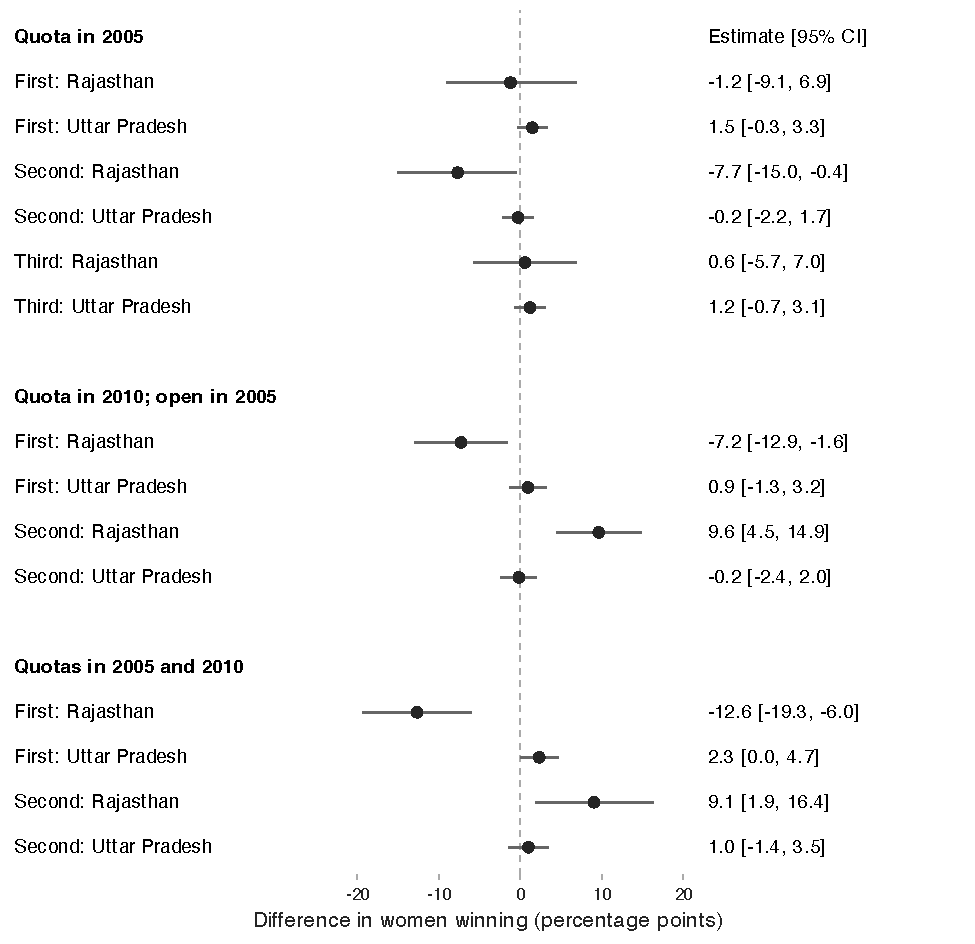
\includegraphics[width=\textwidth]{../figs/persistence_horizons.pdf}
\caption{Women's electoral success across consecutive open elections}
\label{fig:persistence_horizons}
\begin{minipage}{\textwidth}\small
\emph{Notes:} Each group compares the indicated reservation history with offices open in all four observed elections. No women's reservation intervenes during follow-up. Within each state and reservation history, the same GPs contribute at every follow-up; samples differ across histories. Points are block fixed-effects contrasts in the probability that a woman wins, in percentage points. Horizontal lines are pointwise 95\% wild cluster bootstrap intervals. For the first history, follow-up elections are 2010, 2015, and 2020 (Rajasthan) or 2021 (UP); for the other histories, they are 2015 and 2020 or 2021. Sources: the linked Rajasthan and UP election panels described in Appendix~\ref{sec:app_data}.
\end{minipage}
\end{figure}
\FloatBarrier

\begin{table}[!htbp]
\centering
\caption{Reservation histories and later open-election outcomes}
\label{tab:persistence_horizons}

\centering\begingroup\fontsize{8}{10}\selectfont

\resizebox{\ifdim\width>\linewidth\linewidth\else\width\fi}{!}{
\begin{tabular}[t]{llrlrlll}
\toprule
State & History & Election & N (T/C) & Mixed blocks & Women T/C (\%) & Estimate (pp) & 95\% interval\\
\midrule
Rajasthan & 1000--0000 & 2010 & 104/225 & 58 & 8.7/11.1 & -1.2 & {}[-9.1, 6.9]\\
Rajasthan & 1000--0000 & 2015 & 104/225 & 58 & 6.7/12.0 & -7.7 & {}[-15.0, -0.4]\\
Rajasthan & 1000--0000 & 2020 & 104/225 & 58 & 6.7/8.4 & 0.6 & {}[-5.7, 7.0]\\
Rajasthan & 0100--0000 & 2015 & 417/225 & 96 & 6.5/12.0 & -7.2 & {}[-12.9, -1.6]\\
Rajasthan & 0100--0000 & 2020 & 417/225 & 96 & 13.2/8.4 & 9.6 & {}[4.5, 14.9]\\
\addlinespace
Rajasthan & 1100--0000 & 2015 & 219/225 & 75 & 4.1/12.0 & -12.6 & {}[-19.3, -6.0]\\
Rajasthan & 1100--0000 & 2020 & 219/225 & 75 & 15.1/8.4 & 9.1 & {}[1.9, 16.4]\\
Uttar Pradesh & 1000--0000 & 2010 & 3911/2914 & 539 & 15.3/14.2 & 1.5 & {}[-0.3, 3.3]\\
Uttar Pradesh & 1000--0000 & 2015 & 3911/2914 & 539 & 15.7/15.4 & -0.2 & {}[-2.2, 1.7]\\
Uttar Pradesh & 1000--0000 & 2021 & 3911/2914 & 539 & 17.9/17.1 & 1.2 & {}[-0.7, 3.1]\\
\addlinespace
Uttar Pradesh & 0100--0000 & 2015 & 1986/2916 & 507 & 16.8/15.4 & 0.9 & {}[-1.3, 3.2]\\
Uttar Pradesh & 0100--0000 & 2021 & 1986/2916 & 507 & 16.8/17.0 & -0.2 & {}[-2.4, 2.0]\\
Uttar Pradesh & 1100--0000 & 2015 & 1997/2916 & 509 & 18.0/15.4 & 2.3 & {}[0.0, 4.7]\\
Uttar Pradesh & 1100--0000 & 2021 & 1997/2916 & 509 & 18.5/17.0 & 1.0 & {}[-1.4, 3.5]\\
\bottomrule
\end{tabular}}
\endgroup{}

\begin{minipage}{\textwidth}\small
\emph{Notes:} Histories list women's reservation in chronological order across the four elections: 1 denotes reserved, 0 open. T denotes the indicated exposure history; C denotes 0000. Sample sizes and unadjusted female-winner shares refer to the same complete-case GPs at every follow-up within a history comparison. Mixed blocks contain both histories. Estimates include baseline block fixed effects; intervals are pointwise 95\% wild cluster bootstrap intervals. All estimates and intervals are in percentage points. Sources: linked state election panels.
\end{minipage}
\end{table}
\FloatBarrier

\begin{table}[!htbp]
\centering
\caption{Changes in history contrasts across open elections}
\label{tab:persistence_horizon_changes}

\centering\begingroup\fontsize{8}{10}\selectfont

\resizebox{\ifdim\width>\linewidth\linewidth\else\width\fi}{!}{
\begin{tabular}[t]{lllllll}
\toprule
State & History & Comparison & Change (pp) & 95\% interval & Bootstrap p & Holm p\\
\midrule
Rajasthan & 1000--0000 & Second minus first & -6.5 & {}[-17.9, 4.8] & 0.270 & 1.000\\
Rajasthan & 1000--0000 & Third minus first & 1.8 & {}[-8.5, 12.1] & 0.733 & 1.000\\
Rajasthan & 0100--0000 & Second minus first & 16.9 & {}[9.8, 23.9] & $<0.001$ & $<0.001$\\
Rajasthan & 1100--0000 & Second minus first & 21.7 & {}[11.9, 31.6] & $<0.001$ & $<0.001$\\
Uttar Pradesh & 1000--0000 & Second minus first & -1.7 & {}[-4.3, 0.8] & 0.183 & 1.000\\
\addlinespace
Uttar Pradesh & 1000--0000 & Third minus first & -0.3 & {}[-2.8, 2.2] & 0.828 & 1.000\\
Uttar Pradesh & 0100--0000 & Second minus first & -1.1 & {}[-4.1, 1.9] & 0.469 & 1.000\\
Uttar Pradesh & 1100--0000 & Second minus first & -1.3 & {}[-4.4, 1.8] & 0.405 & 1.000\\
\bottomrule
\end{tabular}}
\endgroup{}

\begin{minipage}{\textwidth}\small
\emph{Notes:} Each row tests the change in a history contrast using paired outcomes from the same GPs. A positive value means a larger difference at the later election. Models include baseline block fixed effects and cluster at that level. Intervals are pointwise 95\% wild cluster bootstrap intervals; Holm adjustment covers all eight temporal comparisons in this table. Adjustment concerns changes over time, not all level estimates in Figure~\ref{fig:persistence_horizons}.
\end{minipage}
\end{table}
\FloatBarrier

\subsection{Sensitivity}

Table~\ref{tab:persistence_horizon_sensitivity} separates two sample choices for the 2005 comparison. First, allowing each election's available outcomes within the same histories gives similar estimates to the complete-case analysis. Second, requiring open status only through the election being studied retains more GPs at earlier follow-ups. These estimates also remain small in UP. In Rajasthan, the first-election estimate becomes slightly positive and the second-election estimate becomes less negative. These changing samples cannot by themselves establish how an effect changes over time. The table uses cluster-$t$ intervals for all specifications to keep their uncertainty estimates comparable.

The larger changes in Rajasthan's 0100 and 1100 comparisons do not depend on any single block: removing each block in turn leaves the first-election estimates negative and the second-election estimates positive. This influence check does not resolve the selection assumptions for the histories. The trajectories also share comparison GPs and answer a different question from the next-election contrasts, so they do not enter Appendix~\ref{sec:additional_evidence}'s next-election meta-analysis as additional independent studies.

\begin{table}[!htbp]
\centering
\caption{Sensitivity to follow-up and outcome requirements}
\label{tab:persistence_horizon_sensitivity}

\centering\begingroup\fontsize{8}{10}\selectfont

\resizebox{\ifdim\width>\linewidth\linewidth\else\width\fi}{!}{
\begin{tabular}[t]{llrlll}
\toprule
State & Sample & Election & N (T/C) & Estimate (pp) & Cluster 95\% interval\\
\midrule
Rajasthan & Same GPs & 2010 & 104/225 & -1.2 & {}[-9.1, 6.7]\\
Rajasthan & Available outcomes & 2010 & 105/229 & -2.1 & {}[-10.1, 5.9]\\
Rajasthan & Same GPs & 2015 & 104/225 & -7.7 & {}[-14.9, -0.4]\\
Rajasthan & Available outcomes & 2015 & 105/229 & -7.5 & {}[-14.6, -0.4]\\
Rajasthan & Same GPs & 2020 & 104/225 & 0.6 & {}[-5.5, 6.7]\\
\addlinespace
Rajasthan & Available outcomes & 2020 & 104/225 & 0.6 & {}[-5.5, 6.7]\\
Rajasthan & Open through followup & 2010 & 924/1916 & 1.4 & {}[-0.9, 3.8]\\
Rajasthan & Open through followup & 2015 & 287/619 & -3.6 & {}[-7.3, 0.0]\\
Rajasthan & Open through followup & 2020 & 104/225 & 0.6 & {}[-5.5, 6.7]\\
Uttar Pradesh & Same GPs & 2010 & 3911/2914 & 1.5 & {}[-0.3, 3.3]\\
\addlinespace
Uttar Pradesh & Available outcomes & 2010 & 3911/2914 & 1.5 & {}[-0.3, 3.3]\\
Uttar Pradesh & Same GPs & 2015 & 3911/2914 & -0.2 & {}[-2.2, 1.7]\\
Uttar Pradesh & Available outcomes & 2015 & 3912/2916 & -0.2 & {}[-2.2, 1.7]\\
Uttar Pradesh & Same GPs & 2021 & 3911/2914 & 1.2 & {}[-0.7, 3.1]\\
Uttar Pradesh & Available outcomes & 2021 & 3912/2916 & 1.3 & {}[-0.7, 3.2]\\
\addlinespace
Uttar Pradesh & Open through followup & 2010 & 9311/10251 & 1.3 & {}[0.3, 2.4]\\
Uttar Pradesh & Open through followup & 2015 & 6537/5645 & 0.0 & {}[-1.4, 1.4]\\
Uttar Pradesh & Open through followup & 2021 & 3912/2916 & 1.3 & {}[-0.7, 3.2]\\
\bottomrule
\end{tabular}}
\endgroup{}

\begin{minipage}{\textwidth}\small
\emph{Notes:} All rows compare reservation versus no reservation in 2005. ``Same GPs'' requires open status and observed outcomes at all three subsequent elections. ``Available outcomes'' retains the same reservation histories but requires an outcome only at the displayed election. ``Open through followup'' requires no reservation between 2005 and the displayed election, allowing the sample to vary over time. N (T/C) reports exposed/comparison counts. Estimates include baseline block fixed effects and block-clustered $t$ intervals, in percentage points. Sources: linked state election panels.
\end{minipage}
\end{table}
\FloatBarrier
